\documentclass[9pt]{beamer}
%\documentclass[compress,9pt,usenames,dvipsnames]{beamer}
% \usepackage[utf8]{inputenc}
% \includeonlyframes{current}
\setbeamercovered{dynamic}
\usepackage{etex}
\usepackage{graphicx,url,psfrag}
\usepackage{tikz}
\usetikzlibrary{decorations.pathreplacing,calc,decorations.fractals,through,shapes,patterns,arrows.meta,decorations.pathreplacing,arrows,shapes,}
\usepackage{tikzpeople}
% \usepackage[center]{subfigure}
\usepackage{enumerate}
\usepackage[makeroom]{cancel}
\usepackage{mathtools}
\usepackage{graphbox}
\usepackage{amssymb}
\usepackage{comment}
\excludecomment{codes}
% \usepackage{movie15}
% \usepackage[showframe]{geometry}
% \usepackage{enumitem}

%
% for warning sign
%
\usepackage{pgfplots}
\usepackage{stackengine}
\usepackage{scalerel}
\usepackage{xcolor}
\usepackage{dbt}
\newcommand\dangersign[1][2ex]{%
  \renewcommand\stacktype{L}%
  \scaleto{\stackon[1.3pt]{\color{red}$\triangle$}{\tiny !}}{#1}%
}
% %  The following is to show codes:
\usepackage{listings}
% \usepackage{color}

\usepackage{pifont}% http://ctan.org/pkg/pifont
\newcommand{\cmark}{\ding{51}}%
\newcommand{\xmark}{\ding{55}}%

\definecolor{dkgreen}{rgb}{0,0.6,0}
\definecolor{gray}{rgb}{0.5,0.5,0.5}
\definecolor{mauve}{rgb}{0.58,0,0.82}

\lstset{frame=tb,
  language=Java,
  aboveskip=3mm,
  belowskip=3mm,
  showstringspaces=false,
  columns=flexible,
  basicstyle={\small\ttfamily},
  numbers=none,
  numberstyle=\tiny\color{gray},
  keywordstyle=\color{blue},
  commentstyle=\color{dkgreen},
  stringstyle=\color{mauve},
  breaklines=true,
  breakatwhitespace=true,
  tabsize=3
}
\lstset{language=Python}

\lstset{ %
  language=Python,                     % the language of the code
  basicstyle=\footnotesize,       % the size of the fonts that are used for the code
  numbers=left,                   % where to put the line-numbers
  numberstyle=\tiny\color{gray},  % the style that is used for the line-numbers
  stepnumber=1,                   % the step between two line-numbers. If it's 1, each line
                                  % will be numbered
  numbersep=5pt,                  % how far the line-numbers are from the code
  backgroundcolor=\color{black},  % choose the background color. You must add \usepackage{color}
  showspaces=false,               % show spaces adding particular underscores
  showstringspaces=false,         % underline spaces within strings
  showtabs=false,                 % show tabs within strings adding particular underscores
  frame=single,                   % adds a frame around the code
  rulecolor=\color{black},        % if not set, the frame-color may be changed on line-breaks within not-black text (e.g. commens (green here))
  tabsize=2,                      % sets default tabsize to 2 spaces
  captionpos=b,                   % sets the caption-position to bottom
  breaklines=true,                % sets automatic line breaking
  breakatwhitespace=false,        % sets if automatic breaks should only happen at whitespace
  title=\lstname,                 % show the filename of files included with \lstinputlisting;
                                  % also try caption instead of title
  keywordstyle=\color{blue},      % keyword style
  commentstyle=\color{dkgreen},   % comment style
  stringstyle=\color{mauve},      % string literal style
  escapeinside={\%*}{*)},         % if you want to add a comment within your code
  morekeywords={*,...}            % if you want to add more keywords to the set
}
% \usepackage[usenames,dvipsnames]{color}
% \lstset{
%   language=R,                     % the language of the code
%   basicstyle=\tiny\ttfamily, % the size of the fonts that are used for the code
%   numbers=left,                   % where to put the line-numbers
%   numberstyle=\tiny\color{Blue},  % the style that is used for the line-numbers
%   stepnumber=1,                   % the step between two line-numbers. If it is 1, each line
%                                   % will be numbered
%   numbersep=5pt,                  % how far the line-numbers are from the code
%   backgroundcolor=\color{white},  % choose the background color. You must add \usepackage{color}
%   showspaces=false,               % show spaces adding particular underscores
%   showstringspaces=false,         % underline spaces within strings
%   showtabs=false,                 % show tabs within strings adding particular underscores
%   frame=single,                   % adds a frame around the code
%   rulecolor=\color{black},        % if not set, the frame-color may be changed on line-breaks within not-black text (e.g. commens (green here))
%   tabsize=2,                      % sets default tabsize to 2 spaces
%   captionpos=b,                   % sets the caption-position to bottom
%   breaklines=true,                % sets automatic line breaking
%   breakatwhitespace=false,        % sets if automatic breaks should only happen at whitespace
%   keywordstyle=\color{RoyalBlue},      % keyword style
%   commentstyle=\color{YellowGreen},   % comment style
%   stringstyle=\color{ForestGreen}      % string literal style
% }

% \usepackage[dvipsnames]{xcolor}
% \newcommand{\Cross}{\mathbin{\tikz [x=1.4ex,y=1.4ex,line width=.2ex] \draw (0,0) -- (1,1) (0,1) -- (1,0);}}%
\newcommand{\Crossme}[1]{\!\!
\tikz [black,x=1.1em,y=1.1em,line width=.4ex]
\draw (-0.5,-0.5) -- (0,0) node {\footnotesize #1} -- (0.5,0.5) (0.5,-0.5) -- (-0.5,0.5);}%
\newcommand{\Checkme}[1]{\!\!
\tikz [x=1.1em,y=1.1em,line width=.4ex]
\draw [black] (0,0.7) -- (0.3,0) --(0.9,1.0) (0.5,0.5) node {\footnotesize #1};}
% \beamerdefaultoverlayspecification{<+-| alert@+>} %(this will show line by line)
\beamerdefaultoverlayspecification{<+->} %(this will show line by

% \usepackage{natbib}
% \input{../myMathSymbols.tex}
% \newcommand{\tlMr}[4]{\:{}^{\hspace{0.2em}#1}_{#2} \hspace{-0.1em}#3_{#4}}

% Smiley face\Smiley{} \Frowny{}
\usepackage{marvosym}
% -------------------------------------------------
%  Set directory for figs
% -------------------------------------------------
\usepackage{grffile}
\graphicspath{{Codes/}}
% -------------------------------------------------
%  Define colors
% -------------------------------------------------
\def\refcolor{cyan}
\def\excolor{brown}
% \usepackage{color}
% \usepackage[dvipsnames]{xcolor}


% % % Define danger sign
\newcommand*{\TakeFourierOrnament}[1]{{%
\fontencoding{U}\fontfamily{futs}\selectfont\char#1}}
\newcommand*{\danger}{\TakeFourierOrnament{66}}


% -------------------------------------------------
%  Define short-hand symbols.
% -------------------------------------------------
\newcommand{\B}{\textbf{B}}
\newcommand{\PP}{\mathbb{P}}
\newcommand{\E}{\mathbb{E}}
\newcommand{\D}{\mathbb{D}}
\newcommand{\W}{\dot{W}}
\newcommand{\ud}{\ensuremath{\mathrm{d}}}
\newcommand{\Ceil}[1]{\left\lceil #1 \right\rceil}
\newcommand{\Floor}[1]{\left\lfloor #1 \right\rfloor}
\newcommand{\sgn}{\text{sgn}}
\newcommand{\Lad}{\text{L}_{\text{ad}}^2}
\newcommand{\SI}[1]{\mathcal{I}\left[#1 \right]}
\newcommand{\SIB}[2]{\mathcal{I}_{#2}\left[#1 \right]}
\newcommand{\Indt}[1]{1_{\left\{#1 \right\}}}
\newcommand{\LadInPrd}[1]{\left\langle #1 \right\rangle_{\text{L}_\text{ad}^2}}
\newcommand{\LadNorm}[1]{\left|\left|  #1 \right|\right|_{\text{L}_\text{ad}^2}}
\newcommand{\Norm}[1]{\left|\left|  #1   \right|\right|}
\newcommand{\Ito}{It\^{o} }
\newcommand{\Itos}{It\^{o}'s }
\newcommand{\spt}[1]{\text{supp}\left(#1\right)}
\newcommand{\InPrd}[1]{\left\langle #1 \right\rangle}
\newcommand{\mr}{\textbf{r}}
\newcommand{\Ei}{\text{Ei}}
\newcommand{\arctanh}{\operatorname{arctanh}}
\newcommand{\ind}[1]{\mathbb{I}_{\left\{ {#1} \right\} }}
\newcommand{\Var}{\text{Var}}
\newcommand{\Cov}{\text{Cov}}
\newcommand{\Corr}{\text{Corr}}

\newcommand{\baseurl}[1]{\footnotesize\url{http://math.emory.edu/~lchen41/teaching/2020_Spring/#1}}


\newcommand*\mystrut[1]{\vrule width0pt height0pt depth#1\relax} % adding vertical space

\DeclareMathOperator{\esssup}{\ensuremath{ess\,sup}}

\newcommand{\steps}[1]{\vskip 0.3cm \textbf{#1}}
\newcommand{\calB}{\mathcal{B}}
\newcommand{\calC}{\mathcal{C}}
\newcommand{\calD}{\mathcal{D}}
\newcommand{\calE}{\mathcal{E}}
\newcommand{\calF}{\mathcal{F}}
\newcommand{\calG}{\mathcal{G}}
\newcommand{\calK}{\mathcal{K}}
\newcommand{\calH}{\mathcal{H}}
\newcommand{\calI}{\mathcal{I}}
\newcommand{\calL}{\mathcal{L}}
\newcommand{\calM}{\mathcal{M}}
\newcommand{\calN}{\mathcal{N}}
\newcommand{\calO}{\mathcal{O}}
\newcommand{\calT}{\mathcal{T}}
\newcommand{\calP}{\mathcal{P}}
\newcommand{\calR}{\mathcal{R}}
\newcommand{\calS}{\mathcal{S}}
\newcommand{\calV}{\mathcal{V}}
\newcommand{\bbC}{\mathbb{C}}
\newcommand{\bbN}{\mathbb{N}}
\newcommand{\bbP}{\mathbb{P}}
\newcommand{\bbZ}{\mathbb{Z}}
\newcommand{\myVec}[1]{\overrightarrow{#1}}
\newcommand{\sincos}{\begin{array}{c} \cos \\ \sin \end{array}\!\!}
\newcommand{\CvBc}[1]{\left\{\:#1\:\right\}}
\newcommand*{\one}{{{\rm 1\mkern-1.5mu}\!{\rm I}}}

\newcommand{\OneFrame}[1]{
\begin{enumerate}\item[#1] \phantom{av} \\[20em]\vfill\phantom{av}\myEnd\end{enumerate}}

\newcommand{\bH}{\ensuremath{\mathrm{H}}}
\newcommand{\Ai}{\ensuremath{\mathrm{Ai}}}

\newcommand{\R}{\mathbb{R}}
\newcommand{\myEnd}{\hfill$\square$}
\newcommand{\ds}{\displaystyle}
\newcommand{\Shi}{\text{Shi}}
\newcommand{\Chi}{\text{Chi}}
\newcommand{\Erf}{\ensuremath{\mathrm{erf}}}
\newcommand{\Erfc}{\ensuremath{\mathrm{erfc}}}
\newcommand{\He}{\ensuremath{\mathrm{He}}}
\newcommand{\Res}{\ensuremath{\mathrm{Res}}}

\newcommand{\mySeparateLine}{\begin{center}
 \makebox[\linewidth]{\rule{0.6\paperwidth}{0.4pt}}
\end{center}}

\theoremstyle{definition}
% \newtheorem{definition}[theorem]{Definition}
% \newtheorem{hypothesis}[theorem]{Hypothesis}
\newtheorem{assumption}[theorem]{Assumption}

\theoremstyle{plain}
% \newtheorem{theorem}{Theorem}
% \newtheorem{corollary}[theorem]{Corollary}
% \newtheorem{lemma}[theorem]{Lemma}
\newtheorem{proposition}[theorem]{Proposition}

\mode<presentation>
{
%      \usetheme{Warsaw}
%     \usetheme{JuanLesPins}
%  \usetheme{Hannover}
%  \usetheme{Montpellier}
   \useoutertheme{default}
  % or ...

  \setbeamercovered{transparent}
  % or whatever (possibly just delete it)
 \setbeamertemplate{frametitle}{
  \begin{centering}
    \color{blue}
    {\insertframetitle}
    \par
  \end{centering}
  }
}
\usefoottemplate{\hfill \insertframenumber{}}
% \inserttotalframenumber

\usepackage[english]{babel}
% or whatever

% \usepackage[latin1]{inputenc}
% or whatever

\usepackage{times}
\usepackage[T1]{fontenc}
% Or whatever. Note that the encoding and the font should match. If T1
% does not look nice, try deleting the line with the fontenc.

% \DeclareMathOperator{\Lip}{Lip}
\DeclareMathOperator{\lip}{l}
% \DeclareMathOperator{\Vip}{\overline{v}}
% \DeclareMathOperator{\vip}{\underline{v}}
% \DeclareMathOperator{\vv}{v}
% \DeclareMathOperator{\BC}{BC}
% \DeclareMathOperator{\CH}{CD}

\usepackage{pgfpages}
% \setbeameroption{show notes}
% \setbeamertemplate{note page}[plain]
% \setbeameroption{second mode text on second screen=right}
% \setbeameroption{show notes on second screen=right}
%

% Delete this, if you do not want the table of contents to pop up at
% the beginning of each subsection:
% \AtBeginSubsection[]
% {
%   \begin{frame}<beamer>{Outline}
%     \tableofcontents[currentsection,currentsubsection]
%   \end{frame}
% }

% If you wish to uncover everything in a step-wise fashion, uncomment
% the following command:
% \beamerdefaultoverlayspecification{<+->}

% % % % % % % % % % % % % % % % % % %
%  Define a block
% % % % % % % % % % % % % % % % % % %
\newenvironment<>{problock}[1]{%
  \begin{actionenv}#2%
      \def\insertblocktitle{#1}%
      \par%
      \mode<presentation>{%
        \setbeamercolor{block title}{fg=white,bg=olive!95!black}
       \setbeamercolor{block body}{fg=black,bg=olive!25!white}
       \setbeamercolor{itemize item}{fg=white!20!white}
       \setbeamertemplate{itemize item}[triangle]
     }%
      \usebeamertemplate{block begin}}
    {\par\usebeamertemplate{block end}\end{actionenv}}

\newenvironment<>{assblock}[1]{%
  \begin{actionenv}#2%
      \def\insertblocktitle{#1}%
      \par%
      \mode<presentation>{%
        \setbeamercolor{block title}{fg=white,bg=green!50!black}
       \setbeamercolor{block body}{fg=black,bg=green!10}
       \setbeamercolor{itemize item}{fg=green!80!black}
       \setbeamertemplate{itemize item}[triangle]
     }%
      \usebeamertemplate{block begin}}
    {\par\usebeamertemplate{block end}\end{actionenv}}


% \newtheorem{proofnoend}{Proof.}
% \AtBeginEnvironment{proofnoend}{%
%   \setbeamercolor{block title}{use=example text,fg=lgtblue,bg=background}
%   % \setbeamercolor{block body}{parent=normal text,use=block title example,fg=yellow}
% }

% Define some colors
\definecolor{white}{HTML}{FFFFFF}              % #FFFFFF
\definecolor{pink}{HTML}{FB73BE}               % #FB73BE
\definecolor{coral}{HTML}{FF8D71}              % #FF8D71
\definecolor{yellow}{HTML}{FFE066}             % #FFE066
\definecolor{teal}{HTML}{59F3CE}               % #59F3CE
\definecolor{lgtblue}{HTML}{65D0FA} 	       % #65D0FA
\definecolor{blue}{HTML}{4984F2}               % #4984F2
\definecolor{purple}{HTML}{A87DFF}             % #A87DFF
\definecolor{red}{HTML}{FF3d30}                % #FF3d30
% \definecolor{magenta}{HTML}{FF80FF}                % #FF3d30
\definecolor{green}{HTML}{BBFFB9}              % #BBFFB9
% \definecolor{green}{HTML}{59F3CE}              % #BBFFB9
\setbeamercolor{alerted text}{fg=red}
% \setbeamercolor{block title}{bg=background,fg=lgtblue}

\setbeamercolor{section in toc}{fg=yellow}
\setbeamercolor{subsection in toc}{fg=red}

% \newtheorem{myexample}{\it Example}[section]
\newcounter{myexample}[section]
\resetcounteronoverlays{myexample}
\newenvironment{myexample}[1][]{\refstepcounter{myexample}\par\medskip
\noindent \textbf{\textcolor{green}{Example~\mySecNum-\themyexample~#1}} \rmfamily}{\medskip}

\newcounter{mydefinition}[section]
\resetcounteronoverlays{mydefinition}
\newenvironment{mydefinition}[1][]{\refstepcounter{mydefinition}\par\medskip
\noindent \textbf{\textcolor{yellow}{Definition~\mySecNum-\themydefinition~#1}} \rmfamily}{\medskip}

% \NewCommandCopy{\oldref}{\ref}
% \let\oldref\ref
\newcommand{\myref}[1]{\mySecNum-\ref{#1}}

\newcounter{remark}[section]
\resetcounteronoverlays{remark}
\newenvironment{remark}[1][]{\refstepcounter{remark}\par\medskip
\noindent \textbf{\textcolor{blue}{Remark~\mySecNum-\theremark~#1}} \rmfamily}{\medskip}

\newcounter{mythm}[section]
\resetcounteronoverlays{mythm}
\newenvironment{mythm}[1][]{\refstepcounter{mythm}\par\medskip
\noindent \textbf{\textcolor{lgtblue}{Theorem~\mySecNum-\themythm~#1}} \rmfamily}{\medskip}

\newenvironment{mycor}[1][]{\refstepcounter{mythm}\par\medskip
\noindent \textbf{\textcolor{lgtblue}{Corollary~\mySecNum-\themythm~#1}} \rmfamily}{\medskip}

% \newtheorem{solution}{\textcolor{purple}{Solution}}
\newenvironment{mysol}[1][]{\par\medskip
\noindent \textbf{\textcolor{purple}{Solution#1.~}} \rmfamily}{\medskip}

\newenvironment{myproof}[1][]{\par\medskip
\noindent \textbf{\textcolor{purple}{Proof#1.~}} \rmfamily}{\medskip}

\long\def\script#1{}

% \numberwithin{equation}{section}

% If you have a file called "university-logo-filename.xxx", where xxx
% is a graphic format that can be processed by latex or pdflatex,
% resp., then you can add a logo as follows:

% \pgfdeclareimage[height=1cm]{Emory}{figs/Emory.png}


\title % (optional, use only with long paper titles)
{
  Financial Mathematics \\
  \bigskip
  \small MATH 5870/6870\footnote{\textcolor{gray}{Based on Robert L. McDonald's {\it Derivatives Markets}, 3rd Ed, Pearson, 2013.}}\\
  Fall 2021
}

% \subtitle
% {Research Plan} % (optional)

\author{Le Chen\\[1em]
  {\small\textcolor{gray}{\url{lzc0090@auburn.edu}}}
}


\institute[Auburn University]
{
% \pgfuseimage{Emory}\\[3em]
% {\small Auburn University}\\[1em]
% {\small Auburn AL}\\[3em]
\textcolor{gray}{Last updated on } \\[1em]
\textcolor{gray}{\today}
 \vspace{8em}
}
% - Use the \inst command only if there are several affiliations.
% - Keep it simple, no one is interested in your street address.

\date[Auburn]{Auburn University\\ \textcolor{gray}{Auburn AL}}
% \date{}

% \subject{}



\begin{document}
\begin{frame}[noframenumbering]
  \titlepage
\end{frame}
\newcommand{\myChapter}{Chapter 12. The Black-Scholes Formula}
\newcommand{\mySection}[1]{
  \section{\S\: #1}
  \begin{frame}{\myChapter}\tableofcontents\end{frame}
  \begin{frame}{\myChapter}\tableofcontents[currentsection]\end{frame}
  }
\begin{frame}
\begin{center}
\huge
\myChapter
\end{center}
\end{frame}
\def\mySecNum{12.1}
\mySection{\mySecNum~Introduction to the Black-Scholes formula}
%-------------- start slide -------------------------------%{{{ 1 Limit of Binomial Tree.
\begin{frame}[fragile,t]
\begin{center}

	The \textcolor{magenta}{Black-Scholes formula} is a limiting case of the binomial formula
	(infinitely many periods) for the price of a European option.

	\vfill
	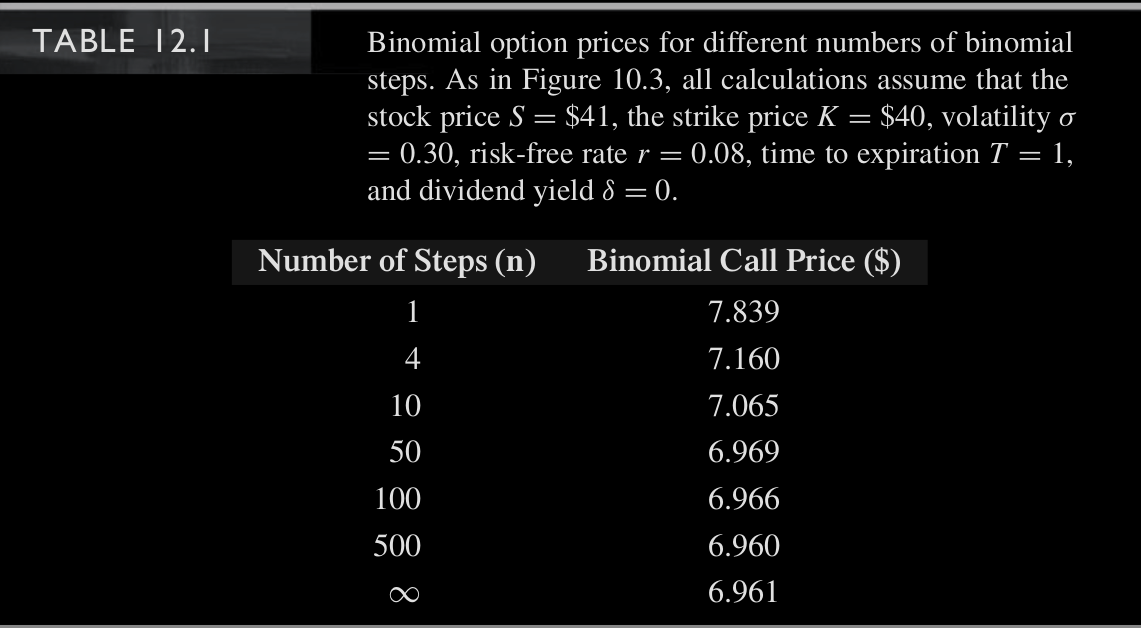
\includegraphics[scale=0.25]{figs/Table-12-1.png}

	\bigskip

	\textcolor{gray}{Check Python code Figure12-1.py}
\end{center}
\end{frame}
%-------------- end slide -------------------------------%}}}
%-------------- start slide -------------------------------%{{{ 1 Formula
\begin{frame}[fragile,t]
	\begin{itemize}
		\item Consider an European call (or put) option written on a stock
		\item Assume that the stock pays dividend at the continuous rate $\delta$
	\end{itemize}
	\pause
	\vfill
	\mySeparateLine

	\begin{minipage}{0.48\textwidth}
	\begin{center}
		Call options
		\begin{gather*}
			C(S,K,\sigma,r,T,\delta) \\ || \\
			S e^{-\delta T}N(d_1)-K e^{-rT}N(d_2)
		\end{gather*}
	\end{center}
	\end{minipage}
	\begin{minipage}{0.48\textwidth}
	\begin{center}
		Put options
		\begin{gather*}
			P(S,K,\sigma,r,T,\delta) \\ || \\
			K e^{-rT}N(-d_2) - S e^{-\delta T}N(-d_1)
		\end{gather*}
	\end{center}
	\end{minipage}
	\bigskip
	\bigskip

	\begin{equation*}
		d_1=\frac{\ln(S/K)+(r-\delta\textcolor{magenta}{+}\frac{1}{2}\sigma^2)T}{\sigma \sqrt{T}} \quad \text{and} \quad
		d_2=\frac{\ln(S/K)+(r-\delta\textcolor{cyan}{-}\frac{1}{2}\sigma^2)T}{\sigma \sqrt{T}}
	\end{equation*}

	\mySeparateLine

	\begin{gather*}
		\text{Put-call Parity}\\
		P = C + Ke^{-rT} - S e^{-\delta T} \\[1em]
		d_1-d_2=\sigma \sqrt{T}
	\end{gather*}
	\bigskip
\end{frame}
%-------------- end slide -------------------------------%}}}
%-------------- start slide -------------------------------%{{{ 1 N(z)
\begin{frame}[fragile,t]
	\begin{align*}
		N(z) = \frac{1}{\sqrt{2\pi}} \int_{-\infty}^z e^{-\frac{x^2}{2}} dx
	\end{align*}
\end{frame}
%-------------- end slide -------------------------------%}}}
%-------------- start slide -------------------------------%{{{ 1 Verification
\begin{frame}[fragile,t]
\begin{myexample}
Verify that the Black-Scholes formula for call and put
\begin{align*}
	C:= C(S,K,\sigma,r,T,\delta) & = S e^{-\delta T}N(d_1)-K e^{-rT}N(d_2) \\
	P:= P(S,K,\sigma,r,T,\delta)  & = K e^{-rT}N(-d_2) - S e^{-\delta T}N(-d_1)
\end{align*}
with
\begin{align*}
	d_i=\frac{\ln(S/K)+(r-\delta\textcolor{magenta}{-(-1)^i}\frac{1}{2}\sigma^2)T}{\sigma \sqrt{T}}, \quad i=1,2
\end{align*}
satisfies the call-put parity: $C - P = S e^{-\delta T} - K e^{-r T}$.
\end{myexample}
\begin{mysol}
	\phantom{a}\\
	\vfill\myEnd
\end{mysol}
\end{frame}
%-------------- end slide -------------------------------%}}}
%-------------- start slide -------------------------------%{{{ 1
\begin{frame}[fragile,t]
	\begin{myexample}
		Plot the functions
		\begin{align*}
			S \to C(S,K,\sigma,r,T-t,\delta) & = S e^{-\delta (T-t)}N(d_1)-K e^{-r(T-t)}N(d_2) \\
			S \to P(S,K,\sigma,r,T-t,\delta)   & = K e^{-r(T-t)}N(-d_2) - S e^{-\delta (T-t)}N(-d_1)
		\end{align*}
		where
		\begin{equation*}
			d_1=\frac{\ln(S/K)+(r-\delta\textcolor{magenta}{+}\frac{1}{2}\sigma^2)(T-t)}{\sigma \sqrt{T-t}} \quad \text{and} \quad
			d_2=\frac{\ln(S/K)+(r-\delta\textcolor{cyan}{-}\frac{1}{2}\sigma^2)(T-t)}{\sigma \sqrt{T-t}}
		\end{equation*}
		with $\sigma, r, \delta, K$ fixed for various values of $T-t=2, 1.5, 1, 0.5, 0$.
	\end{myexample}
	\bigskip
	\begin{mysol}
		Try code \\
		\begin{center}
			\textcolor{gray}{CallPut\_vs\_T-t.nb}
		\end{center}
		\myEnd
	\end{mysol}
\end{frame}
%-------------- end slide -------------------------------%}}}
%-------------- start slide -------------------------------%{{{ 1 Example
\begin{frame}[fragile,t]
\begin{myexample}
	Let $S=\$41$,	$K=\$40$,  $\sigma=0.3$, $r=8\%$,  $T=0.25$ (3 months), and $\delta=0$. Compute the
	Black-Scholes call and put prices. Compare what you obtained with the results obtained from the
	binomial tree.
\end{myexample}
\vfill
\begin{center}
	Check code \\
	\textcolor{gray}{Example12-1.py}
\end{center}
\end{frame}
%-------------- end slide -------------------------------%}}}
%-------------- start slide -------------------------------%{{{ Code -- Removed.
% \begin{frame}[fragile,t]
% 	\begin{center}
% 		\textcolor{gray}{Try code:\\ Example12-1.py}
% 	\end{center}
% 	\bigskip
% 	\begin{lstlisting}
% 	import numpy as np
% 	from scipy.stats import norm
%
% 	# Input the parameters{{{
% 	S = 41
% 	K = 40
% 	sigma = 0.30
% 	r = 0.08
% 	T = 0.25
% 	delta = 0.00
% 	# }}}
%
% 	d1 = (np.log(S/K)+(r-delta+pow(sigma, 2)/2)*T)/(sigma * np.sqrt(T))
% 	d2 = d1 - sigma * np.sqrt(T)
% 	BS_Call = S * np.exp(-delta * T) * norm.cdf(d1) - K * np.exp(-r * T) * norm.cdf(d2)
% 	BS_Put= K * np.exp(- r * T) * norm.cdf(-d2) - S * np.exp(-delta * T) * norm.cdf(-d1)
% 	print("Option prices for call and put computed by Black-Schole model for Examples 12.1 and 12.2 are equal to")
% 	print("{:4.4f} and {:4.4f}, respectively.".format(BS_Call, BS_Put))
% 	\end{lstlisting}
% 	\vfill
% 	\begin{lstlisting}
% 	3.3991 and 1.6070, respectively.
% 	\end{lstlisting}
% \end{frame}
%-------------- end slide -------------------------------%}}}
%-------------- start slide -------------------------------%{{{ 1 Assumptions
\begin{frame}[fragile,t]
	\frametitle{When is the Black-Scholes formula valid?}

	Assumptions about \textcolor{magenta}{stock return distribution}
\bigskip
\begin{itemize}
	\item Continuously compounded returns on the stock are normally distributed and independent over time (no “jumps”)
	\item The volatility of continuously compounded returns is known and constant
	\item Future dividends are known, either as dollar amount or as a fixed dividend yield
\end{itemize}

\pause
\bigskip
\mySeparateLine
\bigskip

Assumptions about the \textcolor{cyan}{economic environment}
\bigskip

\begin{itemize}
	\item The risk-free rate is known and constant
	\item There are no transaction costs or taxes
	\item It is possible to short-sell costlessly and to borrow at the risk-free rate
\end{itemize}
\end{frame}
%-------------- end slide -------------------------------%}}}

\def\mySecNum{12.2}
\mySection{\mySecNum~Applying the formula to other assets}
%-------------- start slide -------------------------------%{{{ 1
\begin{frame}[fragile]
\begin{center}
	This section is left to motivated students to study.
\end{center}
\end{frame}
%-------------- end slide -------------------------------%}}}

\def\mySecNum{12.3}
\mySection{\mySecNum~Option Greeks}
%-------------- start slide -------------------------------%{{{ 1 Intro
\begin{frame}[fragile,t]
	\frametitle{What happens to the option price\\ when one and only one input changes?}

\begin{itemize}
	\item Delta ($\Delta$): change in option price when stock price increases by \$1
	\item Gamma ($\Gamma$): change in delta when option price increases by \$1
	\item Vega: change in option price when volatility increases by 1\%
	\item Theta ($\theta$): change in option price when time to maturity decreases by 1 day
	\item Rho ($\rho$): change in option price when interest rate increases by 1\%
	\item Psi ($\psi$): change in the option premium due to a change in the dividend yield
		\bigskip
		\mySeparateLine
		\bigskip
	\item The \textcolor{magenta}{Greek measure of a portfolio} is weighted average of Greeks of individual portfolio components
		\begin{equation*}
			\Delta_{\text{portfolio}} =\sum_{i=1}^{N} n_i \Delta_i
		\end{equation*}
\end{itemize}
\end{frame}
%-------------- end slide -------------------------------%}}}
%-------------- start slide -------------------------------%{{{ 1
\begin{frame}[fragile]
\begin{center}
	\begin{tikzpicture}[scale=1, transform shape]
		\tikzset{>=latex}
		\node[] (a) at (0,0) {\huge $C(S, K, \sigma, r, T-t,\delta)$};
		\def\len{0.6}
		\draw [<-] (-1.5,0.5) -- ++ (0,\len) node [above] {\huge $\Delta$};
		\draw [<-] (-1.7,0.5+\len+0.3) -- ++ (-\len,0) node [left] {\huge $\Gamma$};
		\draw [<-] (-0.35,-0.3) -- ++ (0,-\len-\len) node [below] {Vega};
		\draw [<-] (0.1,-0.3) -- ++ (0,-\len) node [below] {\huge $\rho$};
		\draw [<-] (1.58,0.5) -- ++ (0,\len) node [above] {\huge $\theta$};
		\draw [<-] (1.98,-0.3) -- ++ (0,-\len) node [below] {\huge $\psi$};
	\end{tikzpicture}
\end{center}
\end{frame}
%-------------- end slide -------------------------------%}}}
%-------------- start slide -------------------------------%{{{ 1 Delta
\begin{frame}[fragile]
	\frametitle{Delta}
	\centering

	\textcolor{magenta}{Delta ($\Delta$)}: change in option price when stock price increases by \$1.
	\bigskip

	\begin{equation*}
		\Delta =
		\begin{cases}
			\displaystyle \frac{\partial C(S,K,\sigma,T-t,\delta)}{\partial S} = +e^{-\delta(T-t)} N(+d_1) & \text{Call} \\[1em]
			\displaystyle \frac{\partial P(S,K,\sigma,T-t,\delta)}{\partial S} = -e^{-\delta(T-t)} N(-d_1) & \text{Put}  \\
		\end{cases}
	\end{equation*}
\end{frame}
%-------------- end slide -------------------------------%}}}
%-------------- start slide -------------------------------%{{{ 1 Proof of Delta
\begin{frame}[fragile,t]
\begin{myexample}
	Demonstrate that
	\begin{equation*}
		\Delta =
		\begin{cases}
			\displaystyle \frac{\partial C(S,K,\sigma,T-t,\delta)}{\partial S} = +e^{-\delta(T-t)} N(+d_1) & \text{Call} \\[1em]
			\displaystyle \frac{\partial P(S,K,\sigma,T-t,\delta)}{\partial S} = -e^{-\delta(T-t)} N(-d_1) & \text{Put}.
		\end{cases}
	\end{equation*}
\end{myexample}
\begin{mysol}
	We only show the call part. By the chain rule:
	\begin{align*}
		\frac{\partial C}{\partial S} = & \quad e^{-\delta (T-t)} N(d_1) \\
                                    & + S e^{-\delta (T-t)} N'(d_1) \frac{\partial d_1}{\partial S} - K e^{-r (T-t)} N'(d_2) \frac{\partial d_2}{\partial S}.
	\end{align*}
	Because $d_2 = d_1 - \sigma \sqrt{T-t}$, we see that
	\begin{align*}
		\frac{\partial d_1}{\partial S} = \frac{\partial d_2}{\partial S}.
	\end{align*}
	It suffices to prove that
	\begin{align*}
		Se^{\delta (T-t)} N'(d_1) = K e^{-r (T-t)} N'(d_2).
	\end{align*}
\end{mysol}
\end{frame}
%-------------- end slide -------------------------------%}}}
%-------------- start slide -------------------------------%{{{ 1 Proof continued
\begin{frame}[fragile,t]
\begin{mysol}( Continued )
	Notice that
	\begin{align*}
		N'(d) = \frac{1}{\sqrt{2\pi}} e^{-\frac{d^2}{2}}.
	\end{align*}
	The above relation is equivalent to
	\begin{align}
		\tag{$\star$}
		\label{E:star}
		\frac{S e^{(r-\delta)(T-t)}}{K} = \exp\left(\frac{d_1^2-d_2^2}{2}\right).
	\end{align}
	Now, from the definitions of $d_1$ and $d_2$, we see that
	\begin{align*}
		d_1^2 - d_2^2 & = d_1^2 - \left(d_1-\sigma \sqrt{T-t}\right)^2 \\
                  & = 2d_1\sigma \sqrt{T-t} - \sigma^2 (T-t)       \\
									& = 2\left(\ln\left(S/K\right) + (r-\delta)(T-t)\right) \\
									& = 2 \ln\left(\frac{Se^{(r-\delta)(T-t)}}{K}\right).
	\end{align*}
	Plugging the above expression back to \eqref{E:star} proves the case. \myEnd
\end{mysol}
\end{frame}
%-------------- end slide -------------------------------%}}}
%-------------- start slide -------------------------------%{{{ 1 Lemma
\begin{frame}[fragile,t]
In the above proof, we have showed the following relation, which will be useful in the computations
of other Greeks:
\bigskip

\begin{align*}
	\huge
	\boxed{S e^{-\delta(T-t)} N'(d_1) = K e^{-r(T-t)} N'(d_2)}
\end{align*}
\end{frame}
%-------------- end slide -------------------------------%}}}
%-------------- start slide -------------------------------%{{{ 1 Graph 12.1
\begin{frame}[fragile]
\begin{center}
	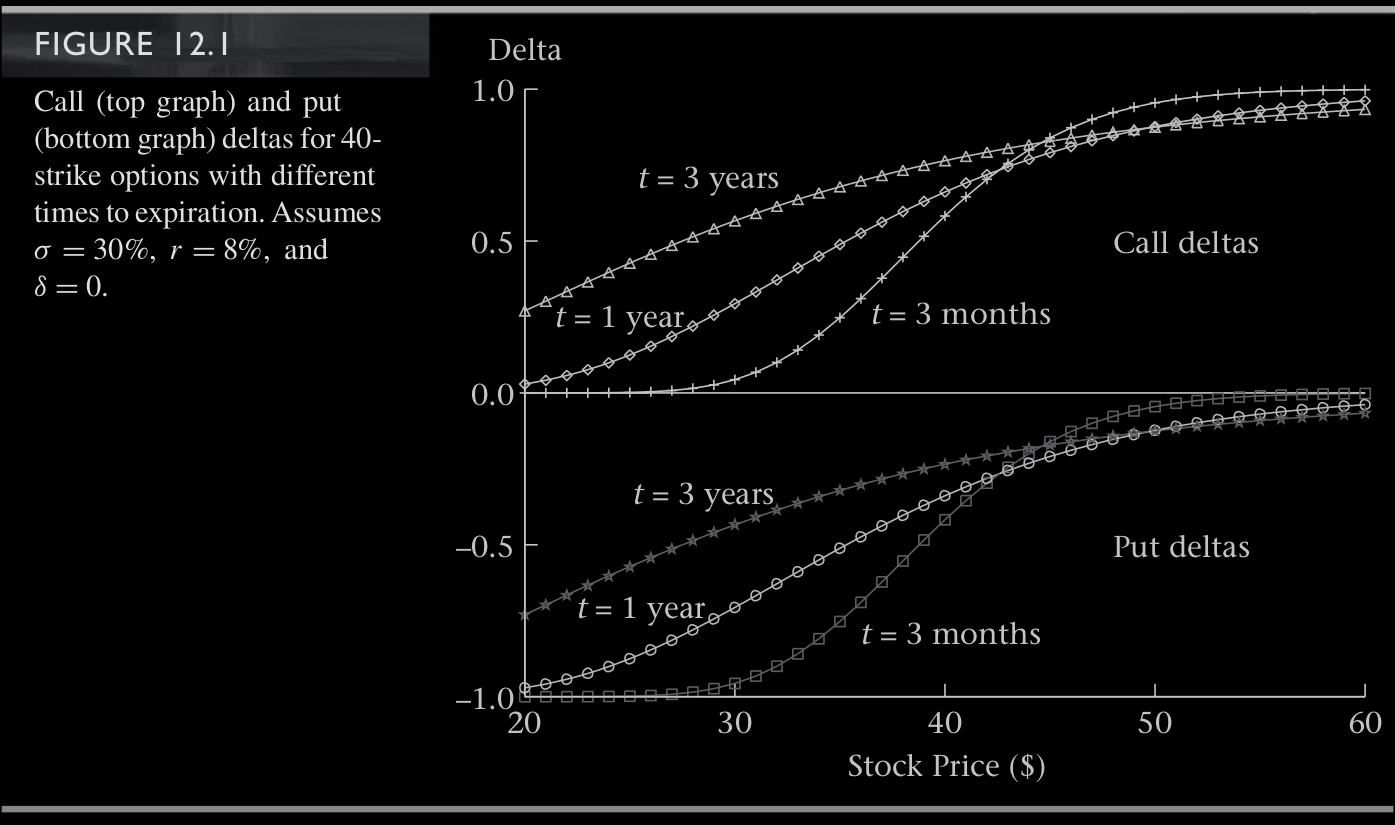
\includegraphics[scale=0.2]{figs/Figure-12-1.png}
\end{center}
\end{frame}
%-------------- end slide -------------------------------%}}}
%-------------- start slide -------------------------------%{{{ 1 Gamma and Vega
\begin{frame}[fragile,t]
	\frametitle{Gamma and Vega}
	\centering

	\textcolor{magenta}{Gamma ($\Gamma$)}: change in delta when option price increases by \$1
	\bigskip

	\begin{equation*}
		\Gamma = \frac{\partial^2 C(S,K,\sigma,r,T-t,\delta)}{\partial S^2}
           = \frac{\partial^2 P(S,K,\sigma,r,T-t,\delta)}{\partial S^2}
           = \frac{e^{-\delta(T-t)N'(d_1)}}{S\sigma \sqrt{T-t}}
	\end{equation*}

	\vfill
	\mySeparateLine
	\vfill

	\textcolor{magenta}{Vega}: change in option price when volatility increases by 1\%
	\bigskip

	\begin{equation*}
		\text{Vega} = \frac{\partial C(S,K,\sigma,r,T-t,\delta)}{\partial \sigma}
                = \frac{\partial P(S,K,\sigma,r,T-t,\delta)}{\partial \sigma}
								= S e^{-\delta (T-t)} N'(d_1) \sqrt{T-t}
	\end{equation*}
\end{frame}
%-------------- end slide -------------------------------%}}}
%-------------- start slide -------------------------------%{{{ 1 Graph 12.2
\begin{frame}[fragile]
\begin{center}
	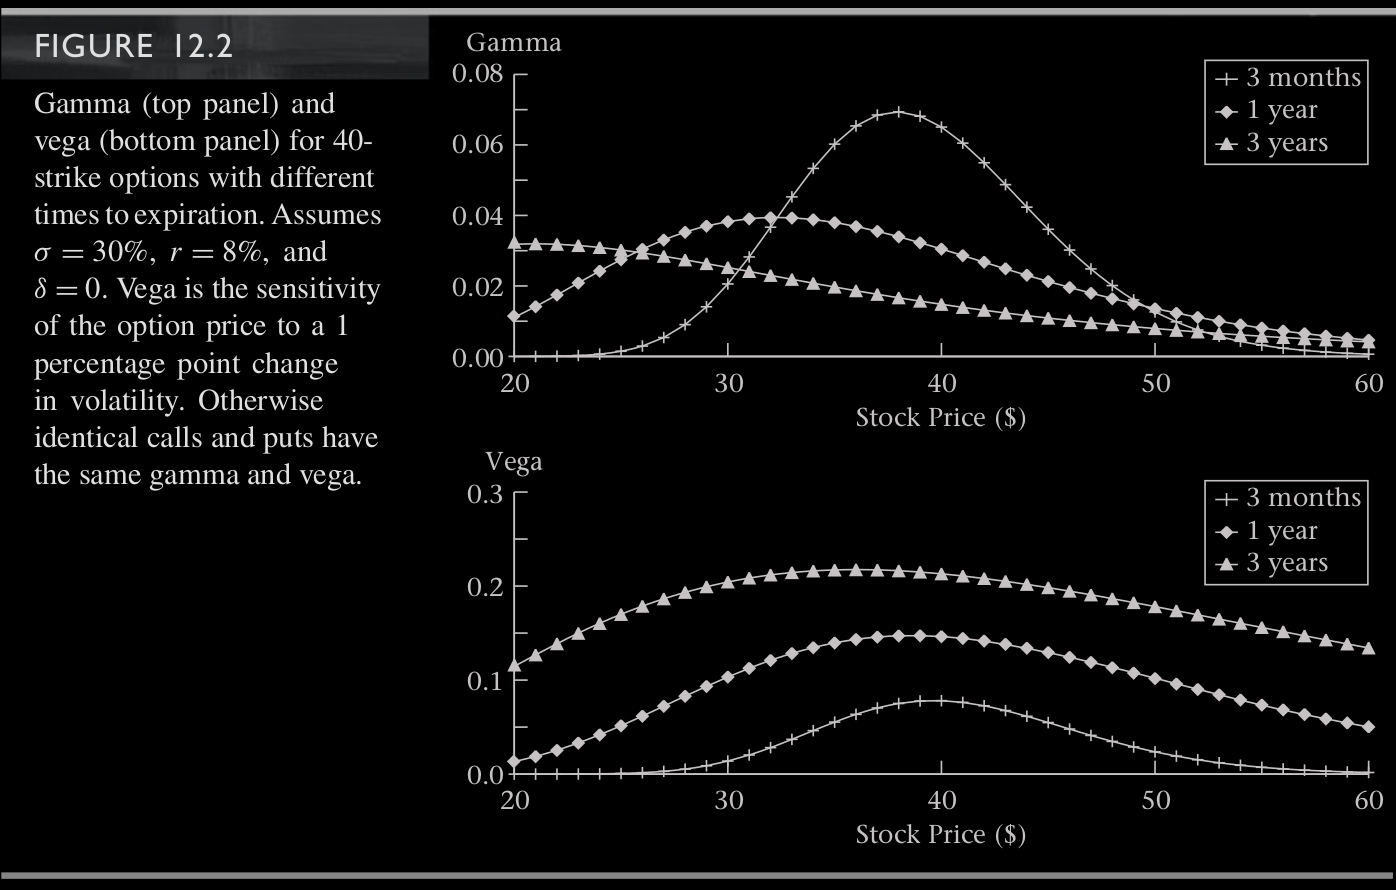
\includegraphics[scale=0.2]{figs/Figure-12-2.png}
\end{center}
\end{frame}
%-------------- end slide -------------------------------%}}}
%-------------- start slide -------------------------------%{{{ 1 Theta
\begin{frame}[fragile]
	\frametitle{Theta}
	\centering

	\textcolor{magenta}{Theta ($\theta$)}: change in option price when time to maturity decreases by 1 day
	\bigskip
	\begin{align*}
		\text{Call $\theta$} & = \frac{\partial C(S,K,\sigma,r,T-t,\delta)}{\partial t}                                              \\
                         & = \delta S e^{-\delta(T-t)}N(d_1)-r K e^{-r(T-t)}N(d_2)- \frac{Ke^{r(T-r)}N'(d_2)\sigma}{2\sqrt{T-t}} \\[1em]
		\text{Put $\theta$}  & = \frac{\partial P(S,K,\sigma,r,T-t,\delta)}{\partial t}                                              \\
                         & = \text{Call $\theta$} + rK e^{-r(T-t)} + \delta S e^{-\delta(T-t)}
	\end{align*}

\end{frame}
%-------------- end slide -------------------------------%}}}
%-------------- start slide -------------------------------%{{{ 1 Graph 12.3
\begin{frame}[fragile]
\begin{center}
	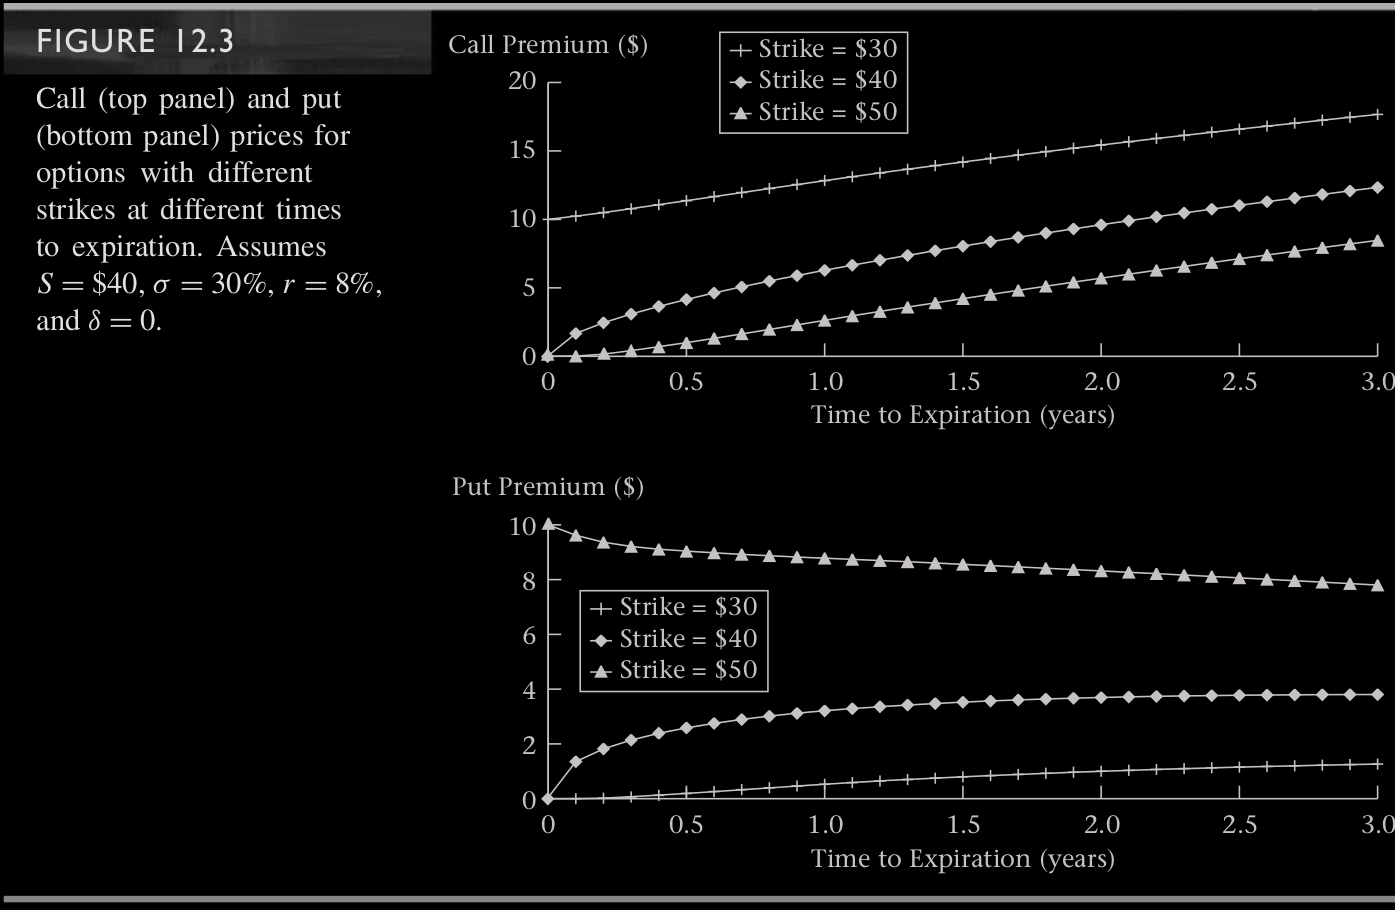
\includegraphics[scale=0.2]{figs/Figure-12-3.png}
\end{center}
\end{frame}
%-------------- end slide -------------------------------%}}}
%-------------- start slide -------------------------------%{{{ 1 Graph 12.4
\begin{frame}[fragile]
\begin{center}
	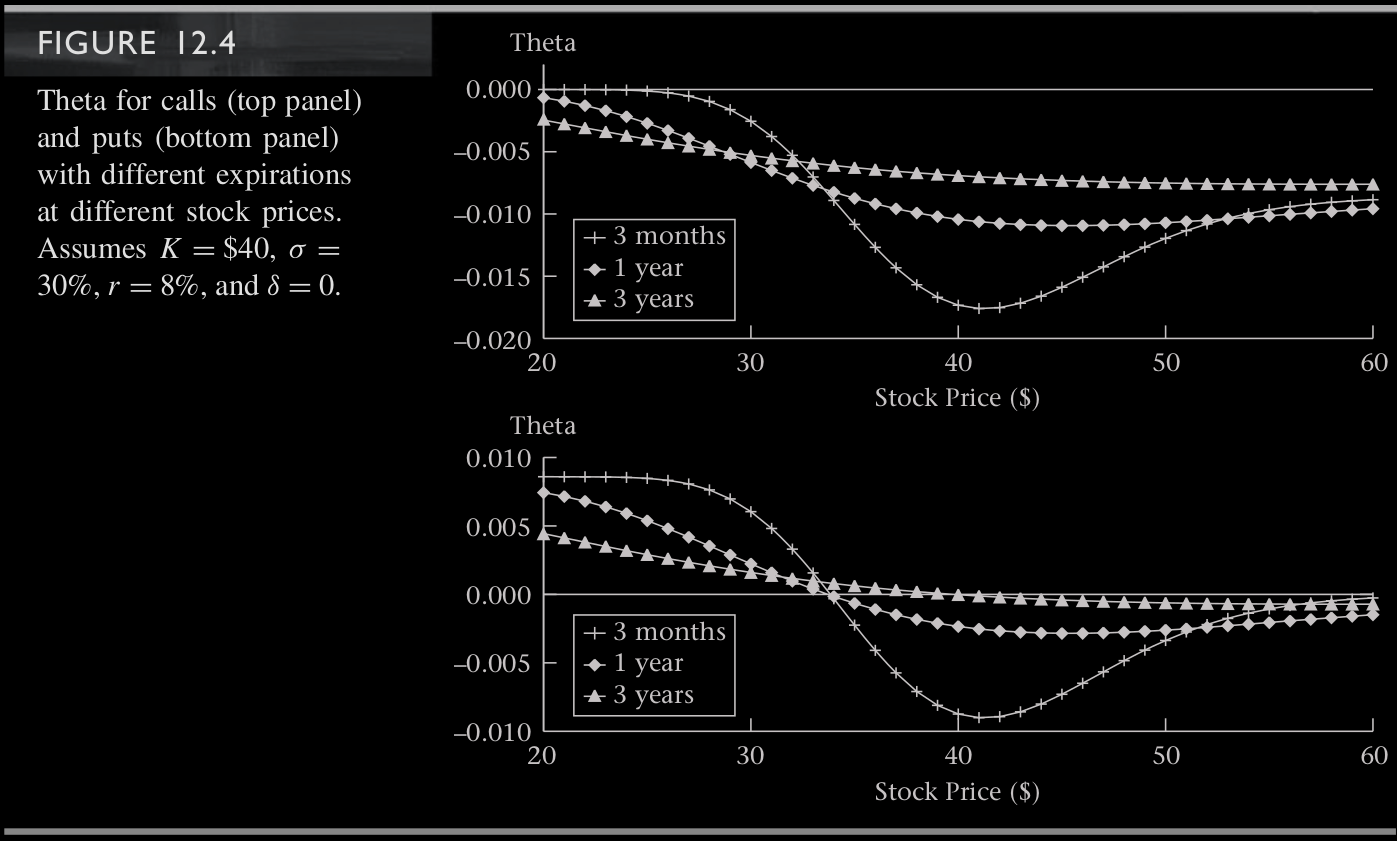
\includegraphics[scale=0.2]{figs/Figure-12-4.png}
\end{center}
\end{frame}
%-------------- end slide -------------------------------%}}}
%-------------- start slide -------------------------------%{{{ 1 Rho and Psi
\begin{frame}[fragile]
	\frametitle{Rho and Psi}
	\centering

	\textcolor{magenta}{Rho ($\rho$)}: change in option price when interest rate increases by 1\%
	\bigskip

	\begin{align*}
		\text{Call $\rho$} & = \frac{\partial C(S,K,\sigma,r,T-t,\delta)}{\partial r} = +(T-t)Ke^{-r(T-t)} N(+d_2) \\
		\text{Put $\rho$}  & = \frac{\partial P(S,K,\sigma,r,T-t,\delta)}{\partial r} = -(T-t)Ke^{-r(T-t)} N(-d_2)
	\end{align*}

	\vfill
	\mySeparateLine
	\vfill

	\textcolor{magenta}{Psi ($\psi$)}: change in the option premium due to a change in the dividend yield

	\begin{align*}
		\text{Call $\psi$} & = \frac{\partial C(S,K,\sigma,r,T-t,\delta)}{\partial \delta} = -(T-t)Ke^{-\delta(T-t)} N(+d_1) \\
		\text{Put $\psi$}  & = \frac{\partial P(S,K,\sigma,r,T-t,\delta)}{\partial \delta} = +(T-t)Ke^{-\delta(T-t)} N(-d_1)
	\end{align*}
\end{frame}
%-------------- end slide -------------------------------%}}}
%-------------- start slide -------------------------------%{{{ 1 Graph 12.5
\begin{frame}[fragile]
\begin{center}
	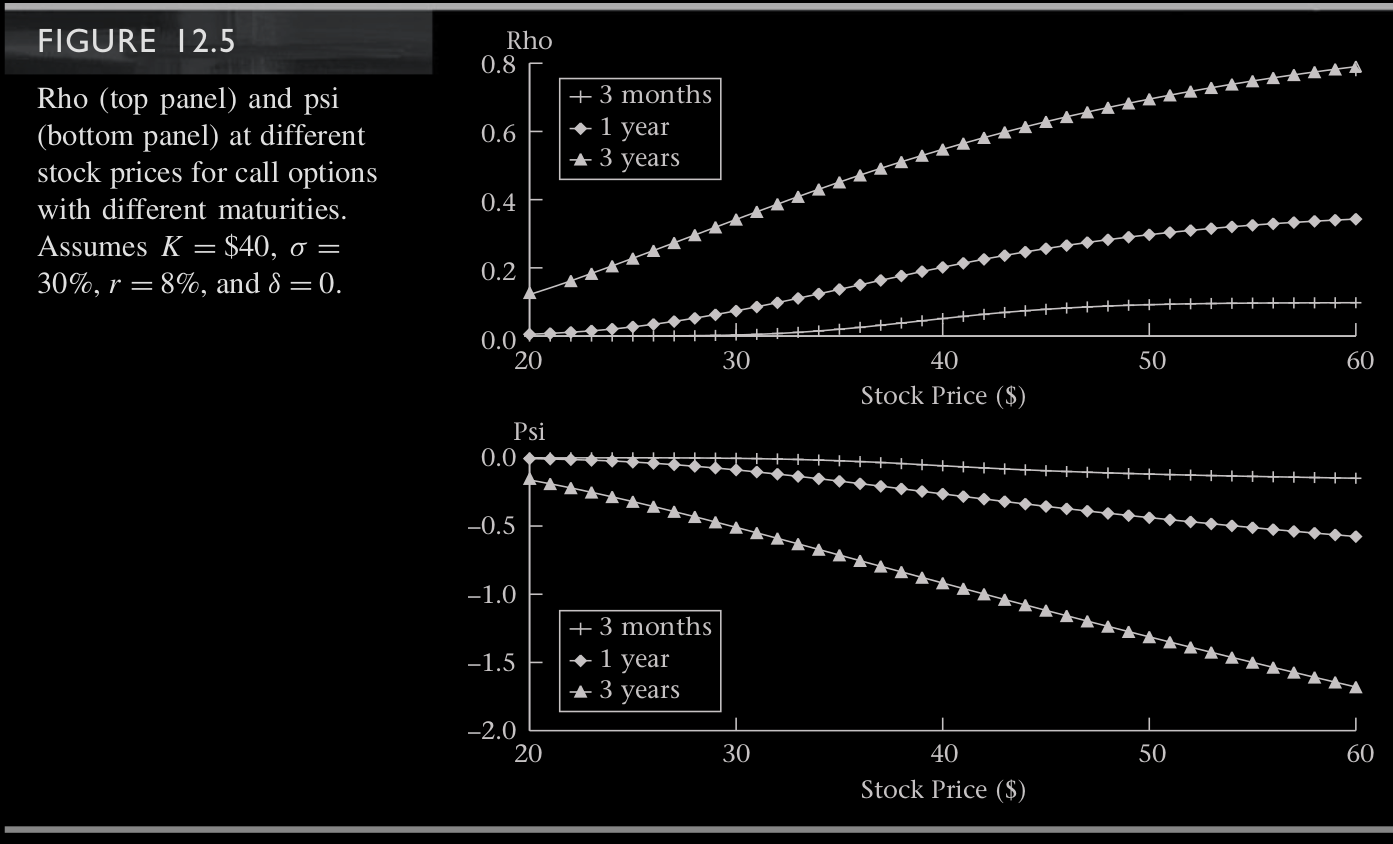
\includegraphics[scale=0.2]{figs/Figure-12-5.png}
\end{center}
\end{frame}
%-------------- end slide -------------------------------%}}}
%-------------- start slide -------------------------------%{{{ 1 Black-Scholes equation
\begin{frame}[fragile,t]
\begin{center}
	Do these Greeks satisfy some relation?
\end{center}
\pause
\bigskip
\mySeparateLine
\bigskip
\begin{mythm}
	Let $V(t,S)$ denote the option price for either European call or put. Recall that
	\begin{align*}
		V_t = \theta, \quad V_S = \Delta, \quad \text{and} \quad V_{SS} = \Gamma.
	\end{align*}
	Then, these three Greeks have to satisfy the \textcolor{magenta}{Black-Scholes equation}:
	\bigskip
	\begin{align}
		\label{E:BSEq}
		\tag{BS}
		\boxed{V_t + \frac{1}{2}\sigma^2 S^2 V_{SS} + (r-\delta) S V_S - r V = 0} \qquad 0 \le t \le T,
	\end{align}
	\bigskip

	with the boundary conditions:
	\bigskip

	\begin{center}
	\renewcommand{\arraystretch}{1.2}
		\begin{tabular}{|c|c|c|}
			\hline
			Condition                  & call          & put             \\ \hline
			$V(T,S)$                   & $\max(S-K,0)$ & $\max(K-S,0)$   \\
			$V(t,S)$                   & $0$           & $K e^{-r(T-t)}$ \\
			$\lim_{S\to\infty} V(t,S)$ & $S$           & $0$             \\ \hline
		\end{tabular}
	\end{center}
\end{mythm}
\end{frame}
%-------------- end slide -------------------------------%}}}
%-------------- start slide -------------------------------%{{{ 1 Proof of BS equation via Mathematica
\begin{frame}[fragile,t]
\begin{myproof}
	We will only verify \eqref{E:BSEq}. This can be easily done by the symbolic computations via
	Mathematica. Check
	\begin{center}
		\textcolor{gray}{Greeks-BS-Equation.nb}
	\end{center}
	\myEnd
\end{myproof}
\end{frame}
%-------------- end slide -------------------------------%}}}
%-------------- start slide -------------------------------%{{{ 1
\begin{frame}[fragile,t]
\begin{center}
	Questions:\\
	\pause
	\bigskip

	(1) How to derive this Black-Scholes equation?\\
	\pause
	\bigskip

	(2) How to solve this equation to get the Black-Scholes formula?
\end{center}
\end{frame}
%-------------- end slide -------------------------------%}}}
%-------------- start slide -------------------------------%{{{ 1 Greek measure of of a portfolio
\begin{frame}[fragile]
	The \textcolor{magenta}{Greek measure of a portfolio} is weighted average of Greeks of individual portfolio components
	\begin{equation*}
		\Delta_{\text{portfolio}} =\sum_{i=1}^{N} n_i \Delta_i
	\end{equation*}
	\vfill
	\begin{center}
		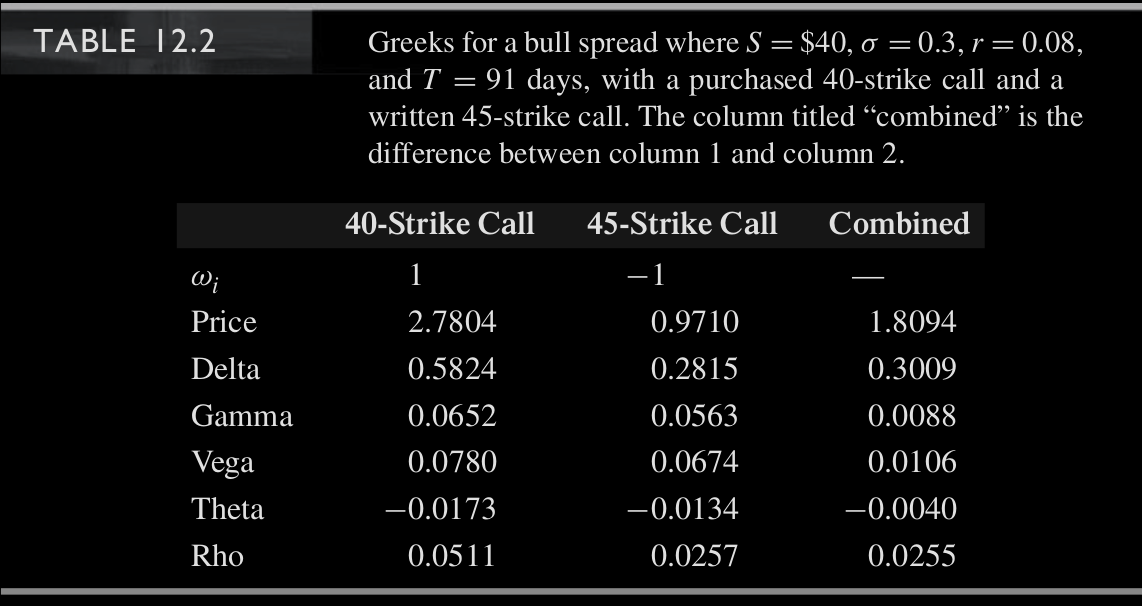
\includegraphics[scale=0.23]{figs/Table-12-2.png}
	\end{center}
\end{frame}
%-------------- end slide -------------------------------%}}}
%-------------- start slide -------------------------------%{{{ 1 Option Elasticity
\begin{frame}[fragile,t]

	\textcolor{cyan}{Delta ($\Delta$)}: change in option price when stock price increases by \$1

	\bigskip
	\mySeparateLine
	\bigskip

	\textcolor{magenta}{Option Elasticity ($\Omega$)}: If stock price $S$ changes by $1\%$, what is
	the percentage change in the value of the option $C$:

	\begin{equation*}
	 \Omega = \frac{\text{Percentage change in option price}}{\text{Percentage change in stock price}}
	 = \frac{\frac{\epsilon \Delta}{C}}{\frac{\epsilon}{S}} = \frac{S\Delta}{C}.
	\end{equation*}
\end{frame}
%-------------- end slide -------------------------------%}}}

\def\mySecNum{12.4}
\mySection{\mySecNum~Problems}
% \mySection{\mySecNum~A. The standard normal distribution}
%-------------- start slide -------------------------------%{{{ 1
\begin{frame}[fragile,t]
	Problems:
	12.3,
	12.4,
	12.6,
	12.7,
	12.9,
	% 12.6,
	% 12.17,
	% 12.18,
	\\
	\bigskip

	Due Date: TBA
\end{frame}
%-------------- end slide -------------------------------%}}}

\end{document}
% \def\mySecNum{12.5}
\mySection{\mySecNum~B. Formulas for option Greeks}
% \def\mySecNum{12.6}
\mySection{\mySecNum~Problems}
